% 3d-two-die-explicit: heat-flow network, EXPLICIT 3D stack (TikZ).
% Source: config/thermal/3d-two-die-explicit.yaml (schema v1.1).
% Compile: pdflatex 3d-two-die-explicit.tex   (TeX Live 2026)
%
% Expanded single-stack form: die_top / die_bottom per-layer nodes,
% inter-layer TSV vertical edge (R_tsv = r_via/n_vias = 50/10 = 5 K/W,
% 10 vias in parallel), top-layer direct cooling vertical chain
% die_top -> ambient (R=1.0 K/W). Every branch annotated with its physical
% path type (conduction) and the value's provenance (YAML). All routing
% orthogonal; sans-serif fonts.
%
% Edge styling: tsv = dashed purple arrow (layer-to-layer conduction);
% vertical_chain = solid amber arrow (conduction). 
\documentclass[border=10pt]{standalone}
\usepackage{sfmath}
\renewcommand{\familydefault}{\sfdefault}
\usepackage{tikz}
\usetikzlibrary{arrows.meta, shapes.geometric}
\definecolor{diefill}{HTML}{E8F0FE}   % die: light blue fill
\definecolor{dieedge}{HTML}{1A73E8}
\definecolor{bndfill}{HTML}{F1F3F4}   % boundary: light gray ellipse
\definecolor{bndedge}{HTML}{5F6368}
\definecolor{tsvedge}{HTML}{9334E6}   % tsv: dashed purple arrow
\definecolor{vcedge}{HTML}{B45309}    % vertical_chain: solid amber arrow
\begin{document}
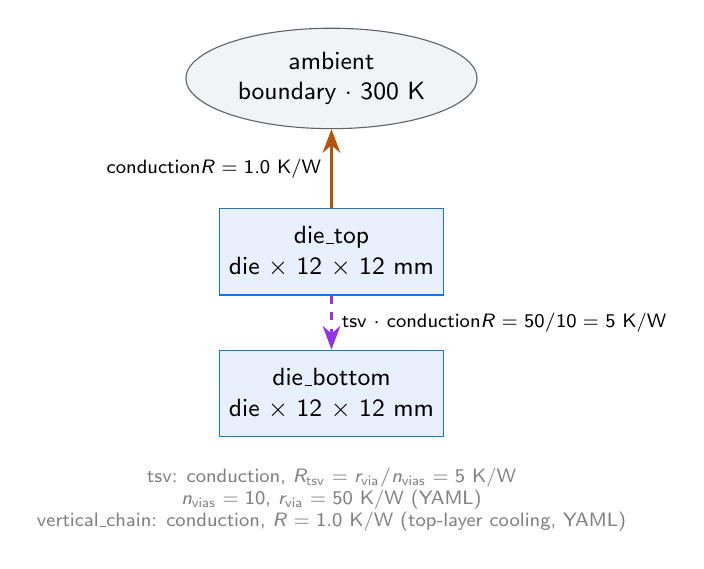
\begin{tikzpicture}[
  die/.style={rectangle, draw=dieedge, fill=diefill, minimum width=2.8cm,
              minimum height=1.1cm, align=center, font=\small},
  bnd/.style={ellipse, draw=bndedge, fill=bndfill, minimum width=3.0cm,
              minimum height=1.1cm, align=center, font=\small},
  tsv/.style={draw=tsvedge, thick, dashed, -{Stealth[length=3mm]}},
  vc/.style={draw=vcedge, thick, -{Stealth[length=3mm]}, rounded corners=0.08cm},
  lab/.style={font=\scriptsize},
]
\node[die] (die_top) at (0,  0.8) {die\_top\\die $\times$ 12 $\times$ 12 mm};
\node[die] (die_bottom) at (0, -1.0) {die\_bottom\\die $\times$ 12 $\times$ 12 mm};
\node[bnd] (ambient) at (0, 3.0) {ambient\\boundary $\cdot$ 300 K};
% inter-layer vertical: TSV (layer-to-layer conduction, vias in parallel)
\draw[tsv] (die_top.south) -- node[right, lab] {tsv $\cdot$ conduction\\$R=50/10=5$ K/W} (die_bottom.north);
% top-layer direct cooling: die_top -> ambient
\draw[vc] (die_top.north) -- node[left, lab] {conduction\\$R=1.0$ K/W} (ambient.south);
% branch annotation: physical path type + value provenance (geometry+material)
\node[lab, align=center, text=gray] at (0, -2.35) {
  tsv: conduction, $R_{\mathrm{tsv}} = r_{\mathrm{via}}/n_{\mathrm{vias}} = 5$ K/W\\
  $n_{\mathrm{vias}}=10$, $r_{\mathrm{via}}=50$ K/W (YAML)\\
  vertical\_chain: conduction, $R=1.0$ K/W (top-layer cooling, YAML)};
\end{tikzpicture}
\end{document}
